%Presentation on numerical differentiation 

\documentclass{beamer}

\mode<presentation>
{
  \usetheme{default}      
  \usecolortheme{default} 
  \usefonttheme{default}  
  \setbeamertemplate{navigation symbols}{}
  \setbeamertemplate{caption}[numbered]
} 

\usepackage[english]{babel}
\usepackage[utf8x]{inputenc}
\usepackage{graphicx}
\usepackage{listings}
\usepackage{color}
\usepackage{setspace}
\usepackage{fancyvrb}

\title[Numerical Differentiation]{Numerical Differentiation}
\author{Omer F Koru and Ethan Feilich}
\institute{University of Pennsylvania}
\date{\today}

\definecolor{mygreen}{rgb}{0,0.6,0}
\lstset{language=Matlab,%
	%basicstyle=\color{red},
	breaklines=true,%
	commentstyle=\color{mygreen}, 
	keywordstyle=\color{blue},%
	numbers=left,%
	numberstyle={\tiny \color{black}},% size of the numbers
	numbersep=9pt, % this defines how far the numbers are from the text
	emph=[1]{for,end,break},emphstyle=[1]\color{red}, %some words to emphasise
	frame=single,
}

%Beginning of presentation

%\setstretch{1.5}

\begin{document}

\begin{frame}
  \titlepage
\end{frame}

\begin{frame}
\frametitle{Basic Concepts}

Why numerical differentiation?\\
\hfill\\

\begin{itemize}
\setlength\itemsep{1em}
\item We have a function we'd like to differentiate, but we only have function values at discrete points
\item We'd like to study changes in data, where it may not be obvious that an underlying function exists
\item Exact formulas for a function may be available, but computationally expensive
\item Discrete approximating solutions to differential equations are defined on a grid, and we need to evaluate derivatives at the grid points
\end{itemize}

\end{frame}

\begin{frame}
\frametitle{Centered Differencing}

\begin{align*}
f'(x) &\approx \frac{f(x+h) - f(x)}{h} & & \textrm{``forward differencing''}\\
f'(x) &\approx \frac{f(x) - f(x-h)}{h} & & \textrm{``backward differencing''}\\
f'(x) &\approx \frac{f(x+h) - f(x-h)}{2h}& & \textrm{``centered differencing''}
\end{align*}

\hfill\\

Centered differencing carries a smaller truncation error which converges ``faster''.

%Centered differencing produces approximation error of order O(h^2) as opposed to other methods where approximation error is of order O(h).

\end{frame}

\begin{frame}
	\frametitle{Error for Different h}
	\begin{figure}
		\centering
			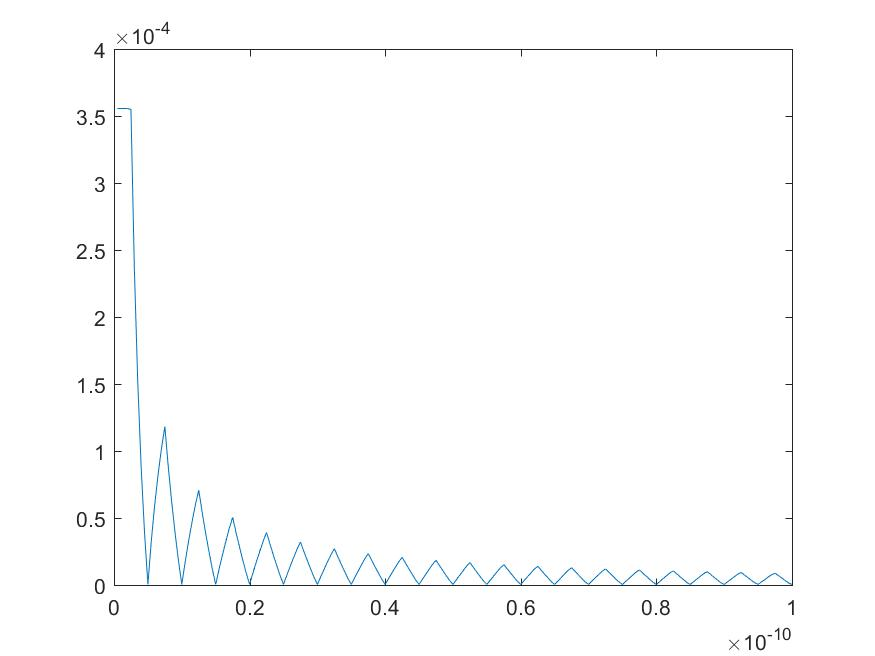
\includegraphics[scale=0.28]{error_diff_sqrt_x}
	\end{figure}
	$f(x) = x^2$, derivative at $2$ with forward differencing
	$h$ from $10^{-12}$ to $10^{-10}$
%	Smaller $h$ higher error!
\end{frame}


\begin{frame}
\frametitle{Optimal Choice of h}

Choose h so as to minimize upper bound on total error.  For forward differencing, that sum is:\\
\begin{align*}
\left\lvert \frac{\widetilde{f(x+h)} - \widetilde{f(x)}}{h}-  f'(x) \right\rvert \leq \frac{4uL_f}{h} + \frac{Mh}{2}
\end{align*}
\begin{align*}
h^* = \sqrt{\frac{uL_f}{M}} \approx \max({\lvert x \rvert , 1}) \sqrt{u}
\end{align*}
\hfill\\
\hfill\\
where $u$ is the ``machine epilon'', $L_f = \sup_{x\in(x,x+h)} |f(x)|$, and $M = \sup_{x\in(x,x+h)} |f''(x)|$

\end{frame}

\begin{frame}
\frametitle{Interpolation}

Assuming we have $f(x_0),\ldots, f(x_n)$, the Lagrange form of the interpolation polynomial is:

\begin{align*}
Q_n(x) = \sum_{j=0}^n f(x_j) l_j(x)
\end{align*}

The numerical differentiation formula, derived from the interpolation error formula is:
%Discuss derivation of this formula from differentiation of interpolation error formula.  

\begin{align*}
f'\left( x_{k}\right) &=\sum _{j=0}^{n}f\left( x_{j}\right) l'_{j}\left( x_{k}\right)+\dfrac {1} {\left( n+1\right) !}f^{\left( n+1\right) }\left( \xi _{x_{k}}\right)  \prod _{\substack{j=0\\j\neq k}}\left( x_{k}-x_{j}\right) \\
%&= Q'_n(x_k) + \dfrac {1} {\left( n+1\right) !}f^{\left( n+1\right) }\left( \xi _{x_{k}}\right)  \prod _{\substack{j=0\\j\neq k}}\left( x_{k}-x_{j}\right)
\end{align*}

where $\xi_{x_k}\in  (min(x, x_0, . . . , x_k), max(x, x_0, . . . , x_k)). $
\end{frame}

\begin{frame}
	\frametitle{Undetermined Coefficients}
	%\setstretch{1.5}
	Centered differencing cannot be used at the boundaries. Interpolation has computational penalty. Another approach:\\
	Suppose we have there data points, $f(x_1), f(x_2), f(x_3)$. \\ \hfill\\
	
	\begin{itemize}
		\setlength\itemsep{1em}
		\item Assume derivative of $f(x_1)$ is linear combination of these points:
		\begin{equation*}
				f^\prime(x_1) \approx af(x_1) + bf(x_2) + cf(x_3)
		\end{equation*}
		\item Derive the Taylor expansions around $x_1$ of $x_i$ for $i=2,3$
		\begin{equation*}
			f(x_i) = f(x_1) + f'(x_1)(x_i - x_1) + \frac{f''(x_1)(x_i-x_1)^2}{2}+\frac{(x_i-x_1)^3 f'''(\xi_i)}{6}
		\end{equation*}
		

	\end{itemize}
	
\end{frame}

\begin{frame}
	\frametitle{Undetermined Coefficients}
	\begin{itemize}
		\setlength\itemsep{1em}
			\item Plug these into the first equation
			\item Equate coefficients on the right hand side to left hand side
			\begin{align*}
				{\color{red}0}\times f(x_1) + & {\color{mygreen}1}\times f^\prime(x_1) +  {\color{blue}0}\times f^{\prime\prime}(x_1) \approx \\ &{\color{red}(a+b+c)} f(x_1) +
				 {\color{mygreen}\left(b(x_2-x_1) + c(x_3-x_1)\right)} f^\prime(x_1) + \\& 	{\color{blue}\left(b(x_2-x_1)^2 + c(x_3-x_1)^2\right)} f^{\prime\prime}(x_1)
			\end{align*}
			\item Gives us 3 equations and 3 unknowns
				\begin{align*}
					a+b+c=0\\
					b(x_2-x_1) + c(x_3-x_1) = 1\\
					b(x_2-x_1)^2 + c(x_3-x_1)^2 = 0 
				\end{align*}
			\item Set $f^\prime(x_1) = af(x_1) + bf(x_2)  + c f(x_3)$
			\item $h = \min_i {|x_1-x_i|} \implies O(h^2)$
	\end{itemize}	
\end{frame}




\begin{frame}
\frametitle{Richardson’s Extrapolation}

%Richardson's extrapolation is a method used to improve approximation accuracy by incorporating additional points, assuming the structure of the error is known.\\
%\hfill\\
We can do better with using more points.  The truncation error from the centered differencing approximation has the form:

\begin{align*}
f'(x) &= \frac{f(x+h) - f(x-h)}{2h} - \left[ {\color{red}\frac{f^{(3)}(x)}{3!} }h^2 + {\color{red}\frac{f^{(5)}(x)}{5!} } h^4 \right] + \ldots \\
&= D(h) + e_2h^2 + e_4 h^4 + \ldots
\end{align*}
\hfill\\ \hfill\\
where the coefficients $e_k$ don't depend on $h$.  

\end{frame}

%\sum_{k=0}^\infty \frac{f^{(k)}(x)}{k!}h^k - \sum_{k=0}^\infty \frac{(-1)^k f^{(k)}(x)}{k!}h^k

\begin{frame}
\frametitle{Richardson’s Extrapolation}

If we also know $x+2h$ and $x-2h$:\\
\begin{align*}
f'(x) &= D(2h) + e_2(2h)^2 + e_4(2h)^4 + \ldots\\
4f'(x) &= 4D(h) + 4e_2(h)^2 + 4e_4(h)^4 + \ldots\\
\end{align*}
Subtracting the two approximations gives:
\begin{align*}
f'(x) = \frac{4D(h) - D(2h)}{3} - 4e_4h^4 + \ldots
\end{align*}

Which eliminates the $e_2h^2$ term from the error.  The resulting fourth order approximation is:

\begin{align*}
f'(x) = \frac{−f(x + 2h) + 8f(x + h) − 8f(x − h) + f(x − 2h)}{12h} + O(h^4)
\end{align*}

\end{frame}

\begin{frame}
\centering
\setstretch{1.5}
\begin{tabular}{ l| c | c}
	\textbf{Method} & \textbf{Efficiency} & \textbf{\# of Points}\\ \hline
	Forward Differencing & O(h) & 1\\
	Backward Differencing & O(h)  & 1\\
	Centered differencing & $O(h^2)$ & 2\\
	Undetermined Coef & $O(h^2)$ & 3\\
	Extrapolation & $O(h^4)$ &4\\
	Lagrange Interpolation & $O(h^{n-1})$ & n
\end{tabular}
\end{frame}

\begin{frame}[fragile]
	\frametitle{Symbolic Differentiation}
If we know the analytic formula, we can directly get the analytic derivative.
Suppose we have a function:
	\begin{equation*}
	g(a) = log(a+5) \times a^2 \times e^{\sqrt{a}}
	\end{equation*}
	\begin{lstlisting}[tabsize=8,basicstyle=\footnotesize]
	% define symbolic variables
	syms a
	% define symbolic function
	g=  log(a+5)*a^2*exp(sqrt(a));
	% differentiate function
	dg = diff(g);
	% display on the screen
	display(dg);
	\end{lstlisting}

	Output:
	\begin{Verbatim}[fontsize=\small]
dg = 2*a*log(a + 5)*exp(a^(1/2))+(a^2*exp(a^(1/2)))/(a + 5)+
     (a^(3/2)*log(a+5)*exp(a^(1/2)))/2
	\end{Verbatim}
%	
\end{frame}

\begin{frame}[fragile]
	If we want to evaluate on a specific point:
	
	\begin{lstlisting}[tabsize=8,basicstyle=\footnotesize]
	% evaluation of diff at x=2
	a=2;
	%substitute a=2 to dg
	eval(subs(dg))
	% or alternative way: turn it into a function
	dg = matlabFunction(dg);
	dg(2)
	\end{lstlisting}
\end{frame}

\end{document}
